\chapter{Experimental Results}
\label{ch: Chapter4}

As part of this project, we developed a working prototype. As explained in Chapter~\ref{ch: Chapter2} section 2, the first mode is the startup menu:

\begin{figure}[H]
    \centering
    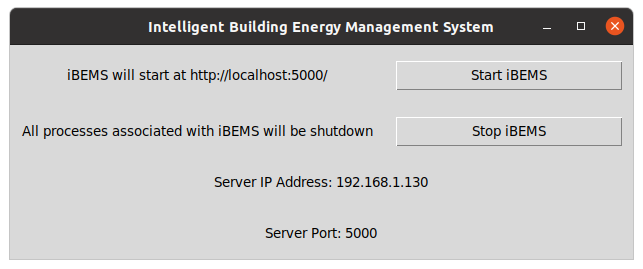
\includegraphics[scale=0.5]{figs/GUI/BEMS_GUI_Linux.png}
    \caption{Desktop GUI}
    \label{fig:desktopgui}
\end{figure}

\noindent
Here, the user will simply click the \say{Start iBEMS} button to launch the web
server and agents. When the user is finished, all agents and the web server can
be shut down by clicking \say{Stop iBEMS}. In case the user accidentally clicks the
\say{Start iBEMS} button while iBEMS is already running, then the following error
message will appear:

\begin{figure}[H]
    \centering
    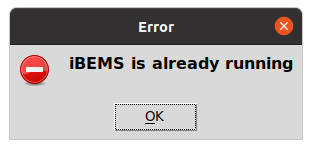
\includegraphics[scale=0.5]{figs/GUI/BEMS_GUI_Linux_Warning.png}
    \caption{Popup Error}
    \label{fig:popuperror}
\end{figure}

\noindent
After launching iBEMS, the web browser will open and the user will presented with the login page:

\begin{figure}[H]
    \centering
    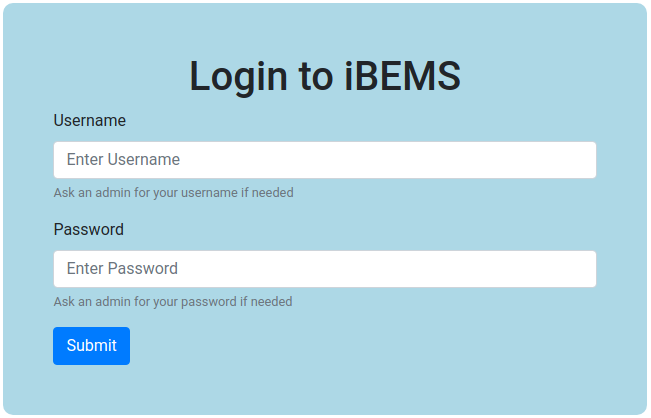
\includegraphics[scale=0.5]{figs/webServer/Login.png}
    \caption{Login Page}
    \label{fig:Home_screen}
\end{figure}

\noindent
where the user can enter in their username and password. Currently, iBEMS does not have a robust user login. It actually just has 1 username and password that is defined in the code. When the user enters the valid username and password, the home page will load automatically, where the weather data can be seen:

\begin{figure}[H]
    \centering
    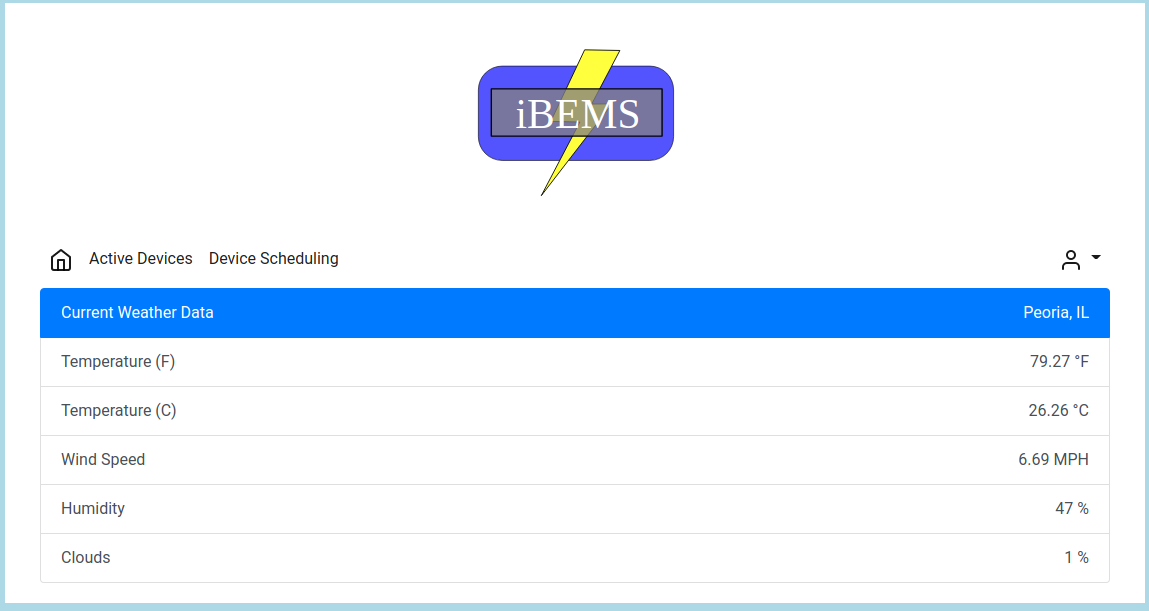
\includegraphics[scale=0.35]{figs/webServer/Home_screen.png}
    \caption{Home Page}
    \label{fig:Home_screen}
\end{figure}

The home screen (mode 2) does not have any interactive functionality other than to load another page by selecting one on the navigation bar.

\begin{figure}[H]
    \centering
    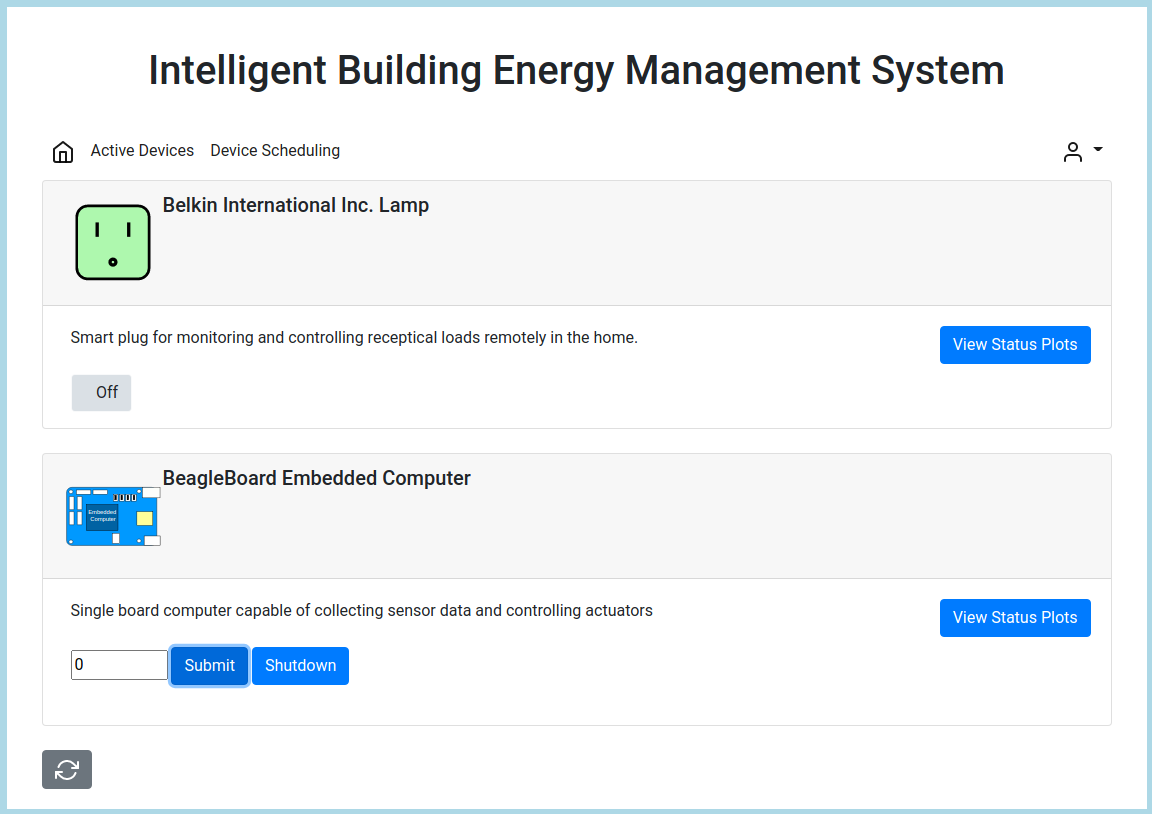
\includegraphics[scale=0.35]{figs/webServer/ActiveDevices_screen.png}
    \caption{Active Devices Page}
    \label{fig:active_devices}
\end{figure}

Figure~\ref{fig:active_devices} shows the active devices page (mode 3) which is loaded upon clicking \say{Active Devices} in the navigation bar. Here, all the connected devices are shown in order of when they connected to iBEMS. As mentioned previously, control of the WeMo Insight Switch is limited to turning it on and off while the embedded computer's motor speed can be controlled by submitting different duty cycles. Additionally, the embedded computer can be completely turned off by clicking the \say{Shutdown} button. Both supported devices also log their power usage at regular intervals. A plot of these power usage data points can be viewed by clicking \say{View Status Plots}.

\begin{figure}[H]
    \centering
    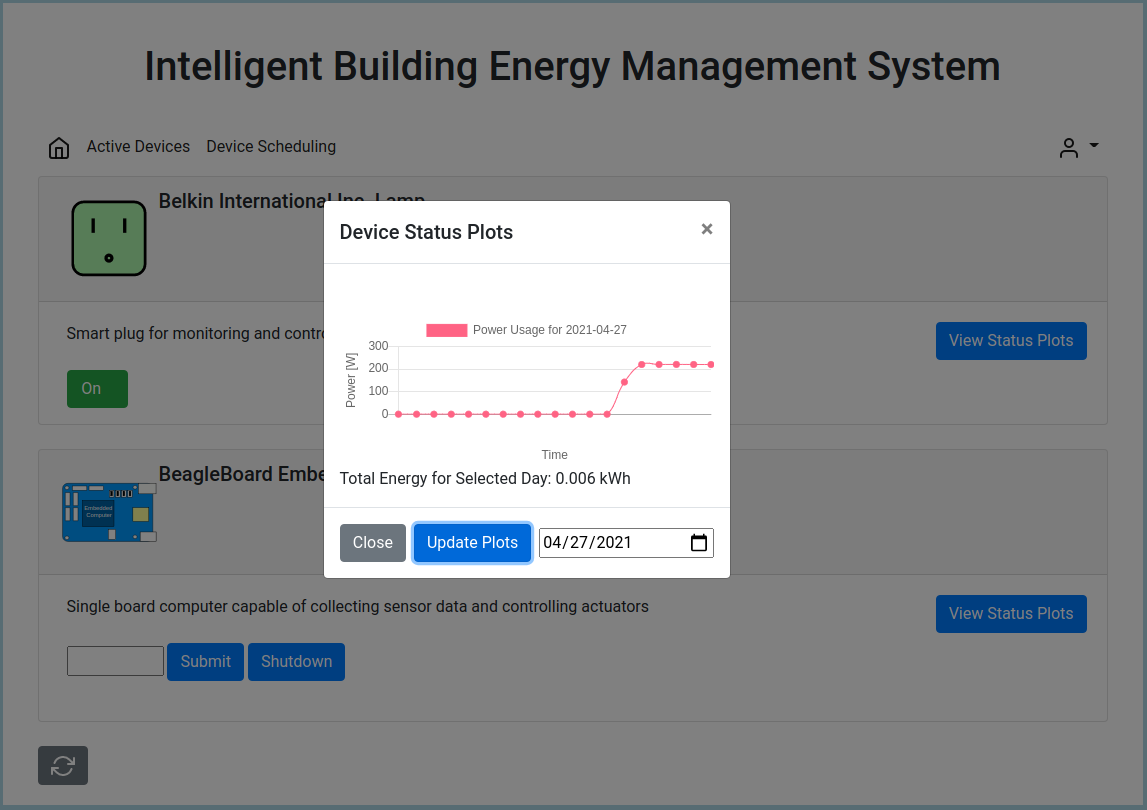
\includegraphics[scale=0.35]{figs/webServer/ActiveDevices_plot.png}
    \caption{Active Devices Plot}
    \label{fig:active_devices_plot}
\end{figure}

After clicking \say{View Status Plots}, a modal will pop up for the user to further
interact with. By default, power usage data points for the current day are
loaded at first, but another day can be selected by clicking on the calendar
icon in the lower right corner. The plot is then updated by clicking \say{Update
Plots}. This is done by collecting data from the Apache Cassandra database and
simply plotting all the points found for the specified day. Underneath the plot,
the total energy consumed for the specified day is displayed. That total energy
is found using the trapezoid method for integration on the plot. %
%
\begin{figure}
    \centering
    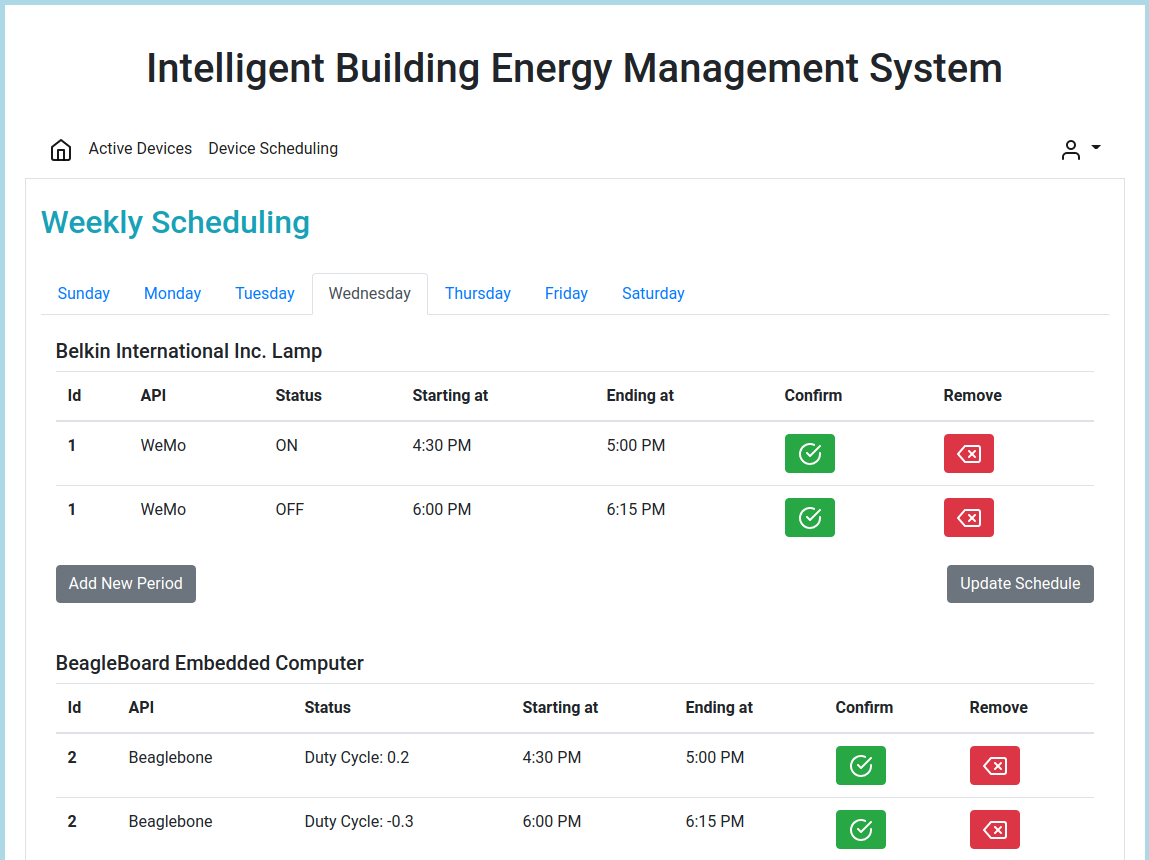
\includegraphics[scale=0.35]{figs/webServer/Applications_screen.png}
    \caption{Scheduling Page}
    \label{fig:schedulingl}
\end{figure}
%

Mode 4, or the scheduling page, can be loaded by clicking the \say{Device
Scheduling} button in the navigation bar. Much like the active devices page,
each connected device is listed in order of when they connected to iBEMS.
Instead of directly controlling the devices, the user can enter in time periods
when they want each device to maintain a specified status. For example, the WeMo
Insight Switch can be scheduled to be on from 5 to 8 P.M. on Fridays. Likewise,
the embedded computer can be scheduled to maintaian a duty cycle of 0.5 for the
same time period every Friday. Scheduled times can be added with the \say{Add new
Period} and deleted by clicking the red \say{X} by the corresponding time period.

%%% Local Variables:
%%% mode: latex
%%% TeX-master: "../finalReport"
%%% End:
